\documentclass[compress]{beamer}
\usefonttheme{professionalfonts}



%

\usepackage[T1]{fontenc}
%\usepackage{kmath,kerkis}
%\usepackage{fouriernc}
\usepackage[adobe-utopia]{mathdesign}
%\usepackage{arev}
\usepackage{times}
\usepackage{natbib}

\usepackage[noend]{algpseudocode}
\usepackage{xmpmulti}
\usepackage{dsfont}
\usepackage{amsmath}

\usepackage{graphicx,float,wrapfig, bbm}
\usepackage{amsfonts, comment, bbold}
\usepackage{mdwlist}
\usepackage{subfigure}
\usepackage{colortbl}
\usepackage{mathrsfs}


\usepackage{multirow}




% packages

\usepackage{amsfonts}

% environments

\newenvironment{packed_enumerate}{
  \begin{enumerate}
    \setlength{\topsep}{0pt}
    \setlength{\itemsep}{2pt}
    \setlength{\parskip}{0pt}
    \setlength{\parsep}{0pt}
}{\end{enumerate}}

\newenvironment{stepit}
 {\begin{itemize}[<+-|alert@+>]}
   {\end{itemize}}

% commands

\newcommand{\Norm}[3]{\mathcal{N}\left( #1, #2, #3 \right)}
\newcommand{\popshow}[2]{\only<#1->{\alert<#1>{#2}}}
\newcommand{\x}{\mathbf{x}}
\newcommand{\ex}[1]{\mbox{exp}\left\{ #1\right\} }
\newcommand{\e}[2]{\mathbb{E}_{#1}\left[ #2 \right] }
\newcommand{\g}{\, | \,}
\newcommand{\indpt}{\protect\mathpalette{\protect\independenT}{\perp}}
\def\independenT#1#2{\mathrel{\rlap{$#1#2$}\mkern2mu{#1#2}}}
\newcommand{\E}{\textrm{E}}
\newcommand{\R}{\textrm{R}}
\newcommand{\realline}{\mathbb{R}}
\newcommand{\data}{{\cal D}}
\newcommand{\loglik}{{\cal L}}
\newcommand{\grad}[2]{ \frac{\partial{#1}}{\partial#2}}
\newcommand{\dir}[1]{\mbox{Dir}(#1)}
\newcommand{\mult}[1]{\mbox{Mult}( #1)}
\newcommand{\G}[1]{\Gamma \left( \textstyle #1 \right)}
\newcommand{\ind}[1]{\mathds{1}\left[ #1 \right] }
\newcommand{\norm}[1]{\left\lVert#1\right\rVert}

\newcommand{\class}[1]{ \texttt{#1}}
\newcommand{\term}[1]{ ``#1''}
\newcommand{\tcword}[0]{ w }
\newcommand{\docsetlabeled}[0]{ D }
\newcommand{\onedoclabeled}[0]{ d }
\newcommand{\tcposindex}[0]{ i }
\newcommand{\myblue}[1]{ {\textbf #1 }}
\newcommand{\dnrm}[1]{ _{\mbox{\textsc{ #1 }}}}
\newcommand{\argmax}[0]{ \arg \max }
\newcommand{\tcjclass}[0]{c_j}
\newcommand{\maths}[1]{ {\bf #1}}




% complexity
\renewcommand{\O}{\mathcal{O}}



\setbeamersize{text margin left=0.5cm}
\setbeamersize{text margin right=0.5cm}
\setbeamercolor{alert}{fg=red!75!black}

\usetheme{default}
\useinnertheme{circles}
\useoutertheme{split}
\usecolortheme{seahorse}
% \usecolortheme{dove}
% \usecolortheme{seagull}
%\usecolortheme{default}
% \usecolortheme{dolphin}
\usefonttheme{structurebold}
%\usefonttheme{serif}

\setbeamertemplate{navigation symbols}{}
\setbeamertemplate{headline}{}
\setbeamertemplate{footline}{}
\setbeamerfont{itemize/enumerate subbody}{size=\normalsize}
\setbeamerfont{itemize/enumerate subsubbody}{size=\normalsize}
\setbeamercolor{itemize item}{fg=gray}
\setbeamercolor{enumerate item}{fg=gray}
\setbeamercolor{itemize item}{fg=gray}
\setbeamercolor{itemize subitem}{fg=gray}
\setbeamercolor{item projected}{bg=gray}
\setbeamercolor{subitem projected}{bg=gray}


\newenvironment{bullets}
{\begin{itemize} \setlength{\itemsep}{10pt}}
{\end{itemize}}

\newcommand{\mygraphic}[2]{
  \begin{beamercolorbox}[colorsep*=4pt]{black math}
    \begin{center}
      \includegraphics[#1]{#2}
    \end{center}
  \end{beamercolorbox}
}

\setbeamercolor{structure}{bg=gray}
\setbeamercolor{section in head/foot}{bg=gray}
\setbeamercolor{palette primary}{bg=lightgray}


\usepackage{minted}

\usetheme[pageofpages=of,                    % String used between the current page and the
                                             % total page count.
          bullet=circle,                     % Use circles instead of squares for bullets.
          titleline=true,                    % Show a line below the frame title.
          showdate=true,                     % show the date on the title page
          alternativetitlepage=true,         % Use the fancy title page.
          titlepagelogo=../../common/culogo,              % Logo for the first page.
          % Logo for the header on first page.
          headerlogo=../../common/boulder_cs,
          ]{UCBoulder}

\usecolortheme{ucdblack}
\author{Introduction to Data Science Algorithms}


\institute[Boyd-Graber and Paul] % (optional, but mostly needed)
{Jordan Boyd-Graber and Michael Paul}


\AtBeginSection[] % "Beamer, do the following at the start of every section"
{ \begin{frame} \frametitle{Outline} % make a frame titled "Outline"
\tableofcontents[currentsection] % show TOC and highlight current section
\end{frame} }

\newcommand{\gfx}[2]{
\begin{center}
	\includegraphics[width=#2\linewidth]{spectral/#1}
\end{center}
}
\title{Spectral Methods}
\date{Anchor Topic Models}

\usepackage[absolute,overlay]{textpos}


\usepackage{colortbl}
\usepackage{subfigure}
\usepackage{bm}
\usepackage{comment}
\usepackage{multirow}
\usepackage{multicol}
\usepackage{natbib}

\usepackage{tabularx}
\usepackage{environ}
\usepackage{dsfont}
\usepackage{textcomp}
\usepackage{float}
\usepackage{graphicx}
\usepackage{mathtools}
\usepackage{mdwlist}
\usepackage{microtype}
\usepackage{amsmath}
\usepackage{caption}
\newcommand{\hidetext}[1]{}

\newcommand{\abr}[1]{\textsc{#1}}
\newcommand{\grammar}[1]{{\color{red} #1}}
\newcommand{\kl}[2]{D_{\mbox{\textsc{KL}}} \left( #1 \,||\, #2 \right)}
\newcommand{\slfrac}[2]{\left.#1\middle/#2\right.}
\newcommand{\cd}[1]{\bar{\bm{Q}}_{#1, \cdot}  }
\newcommand{\tb}[1]{\parbox{0.8\linewidth}{ \scriptsize{ #1 }} \vspace{.2cm} }
\newcommand{\nchooser}[2]{\big(\!\begin{smallmatrix} #1\\#2\end{smallmatrix}\!\big)}

\newcommand{\lda}[0]{{\bf \textsc{\large{lda}}}}
\newcommand{\medlda}[0]{{\bf \textsc{medlda}}}
\newcommand{\slda}[0]{{\bf \textsc{\large{slda}}}}
\newcommand{\ank}[0]{{\bf \textsc{\large{anchor}}}}
\newcommand{\sank}[0]{{\bf \textsc{\large{sup~anchor}}}}
\newcommand{\tfidf}[0]{{\bf \textsc{\large{tf-idf}}}}

\newcommand{\unsupmat}[1]{\bar{Q}_{#1}}
\newcommand{\unsuprow}[1]{\bar{Q}_{#1, \cdot}}
\newcommand{\supmat}[1]{S_{#1}}
\newcommand{\suprow}[1]{S_{#1, \cdot}}
\newcommand{\coef}[1]{C_{#1}}
\newcommand{\topicmat}[1]{A_{#1}}



\newcommand{\red}[1]{{\color{red}{\bf #1}}}
\newcommand{\blue}[1]{{\color{blue}{\bf #1}}}
\newcommand{\green}[1]{{\color{green}{\bf #1}}}
\newcommand{\purple}[1]{{\color{purple}{\bf #1}}}

\begin{document}

\frame{\titlepage
Slides adapted from Thang Nguyen
}

\begin{frame}{What are Spectral Methods}

\begin{itemize}
  \item Bayesian and deep models had explicit generative models
  \item Is it possible to find useful structure from matrix
    representations of data directly?
  \item Spectral methods: often very fast, but hard to engineer
  \item Like last week, a little out of place
  \item Today:
    \begin{itemize}
      \item Anchor Words for Topic Models
      \item Tensors
        \pause
        \item Projects / Presentations
        \item FCQ
    \end{itemize}
\end{itemize}

\end{frame}

\begin{frame}
\frametitle{Anchor Method: Definition}
\begin{figure}[t!]
\centering
\only<1>{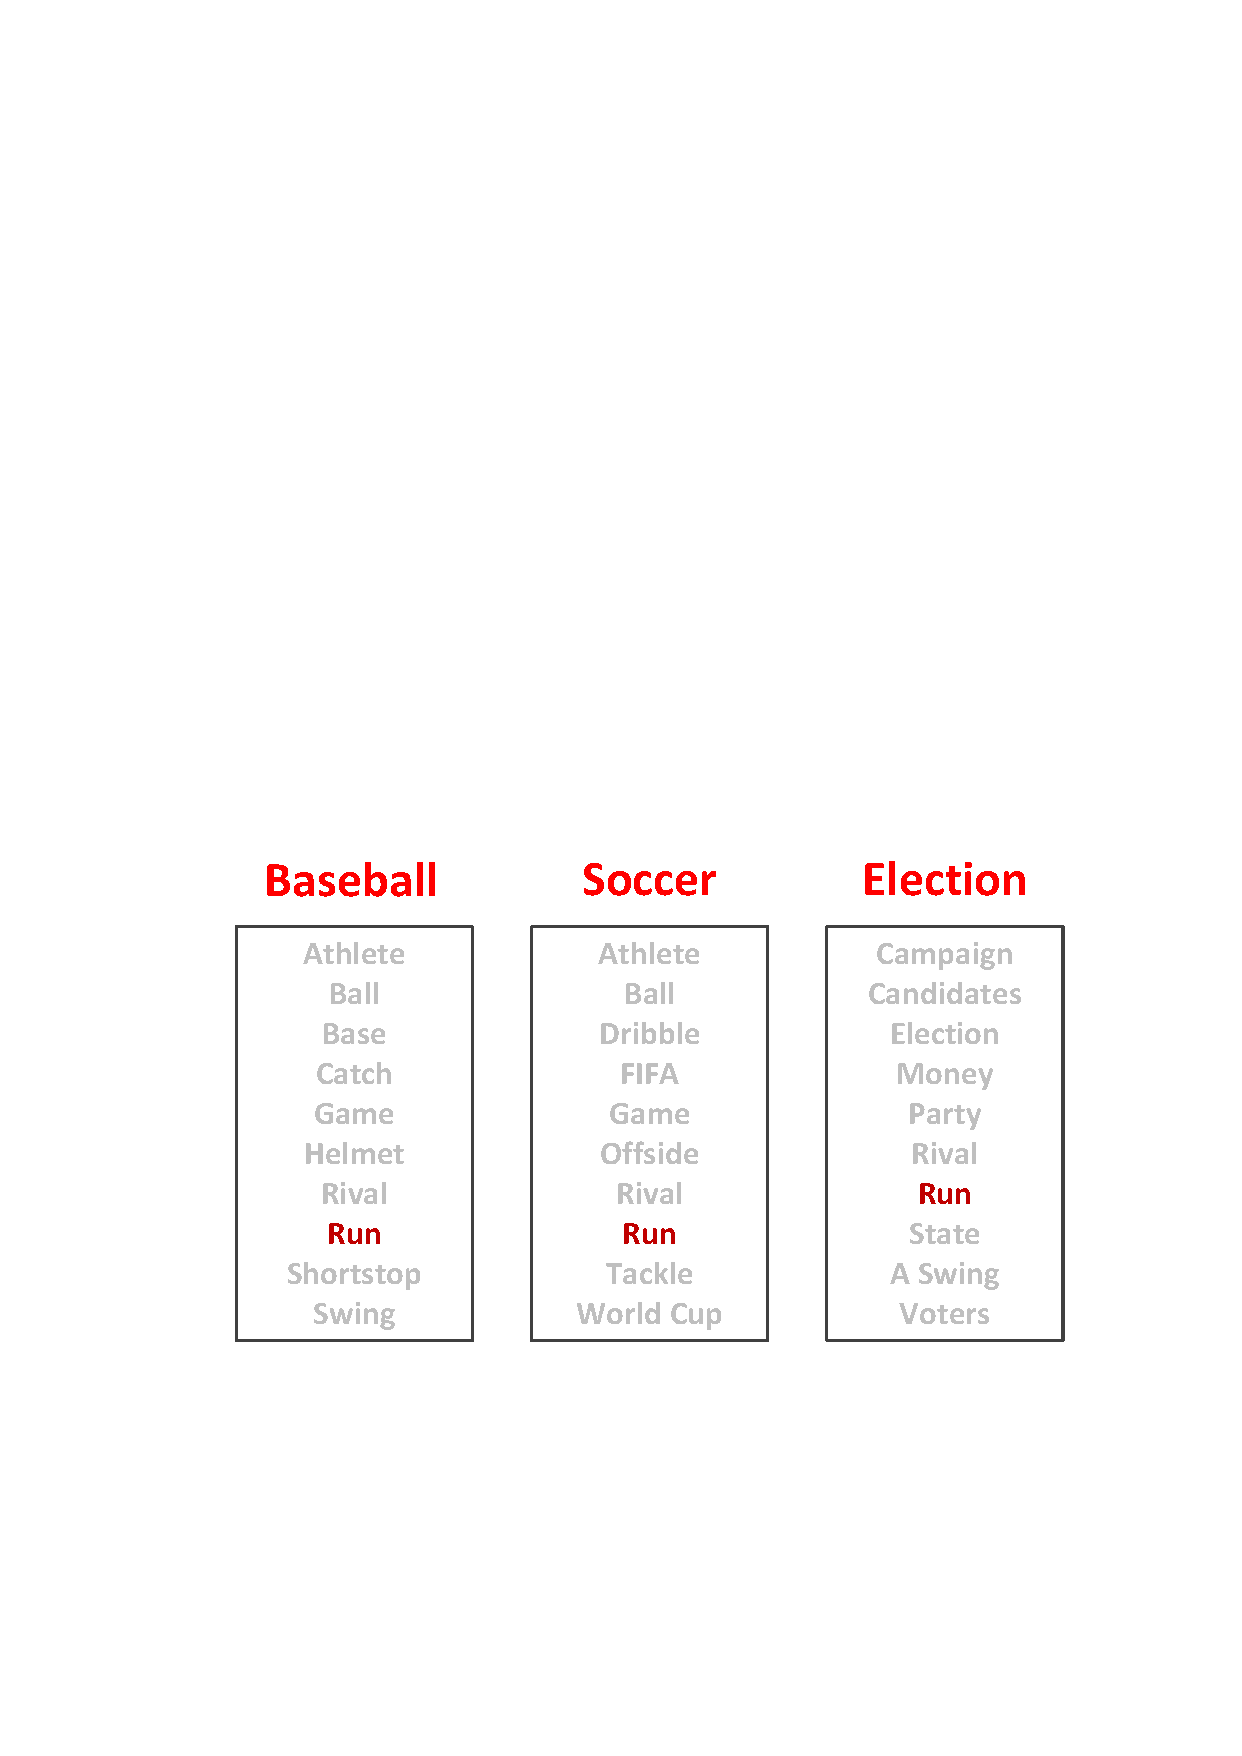
\includegraphics[width=0.8\linewidth]{spectral/Anchor_words_1}}
\only<2>{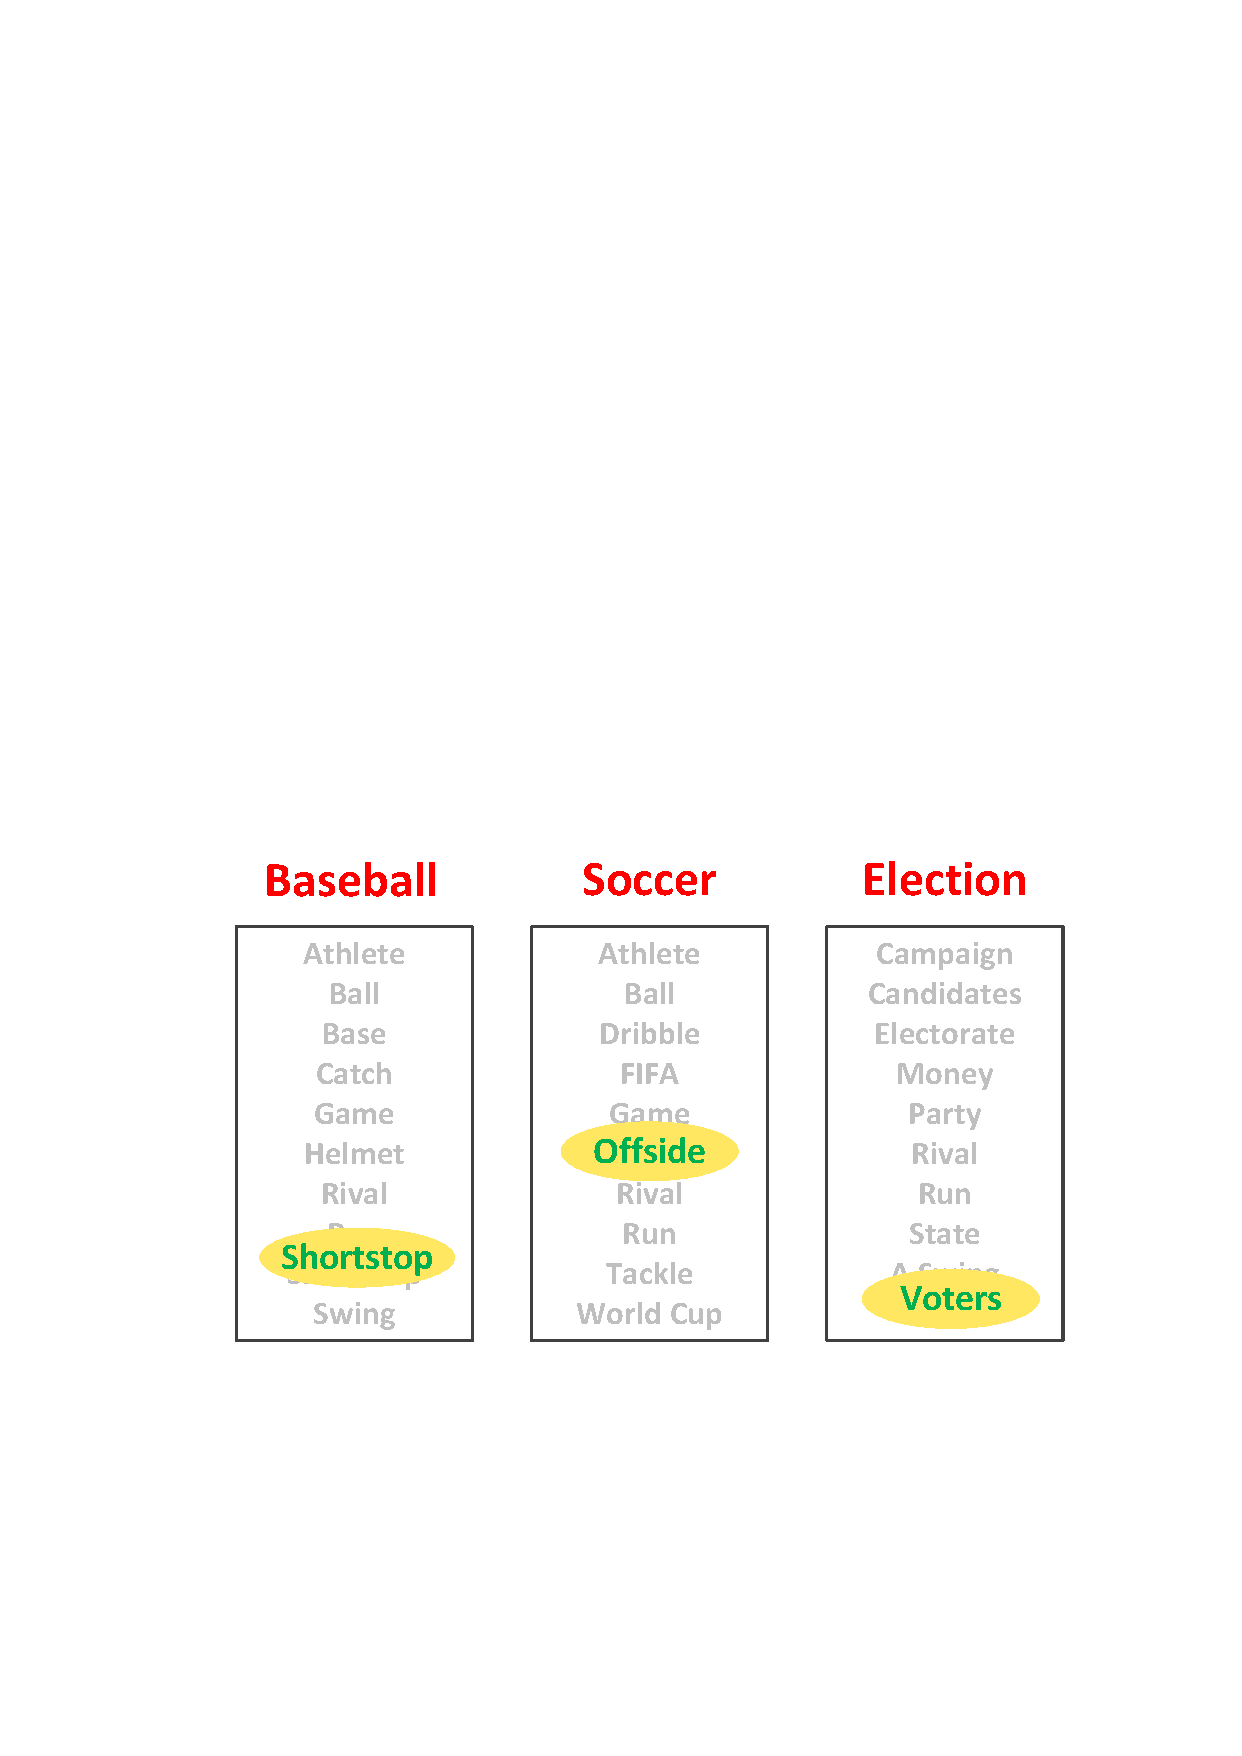
\includegraphics[width=0.8\linewidth]{spectral/Anchor_words_2}}
\label{fig:anchorwords1}
\end{figure}
\Large{
\begin{itemize}
\item Words are often shared among many topics
\item <2>\alert{Anchor words}: words that unique to a topic
\end{itemize}
}
\end{frame}


\begin{frame}{Anchor Method: Big Idea}
\begin{itemize}
  \item Normally, we want to find $p(\mbox{word}|\red{topic})$
 \begin{equation*}
      A_{i,k} = \mbox{p(word = i}|\mbox{topic = \red{k})}
    \end{equation*}
  \item What we'll do instead is find $p(\red{topic}|\mbox{word})$ (topic coefficient)
    \begin{equation*}
      C_{i,k} = \mbox{p(topic = \red{k}} | \mbox{word = i)}
    \end{equation*}
  \pause
  \item Easy: Bayes rule
\end{itemize}

\end{frame}

\begin{frame}{Anchor Method: Why go backward?}

\begin{itemize}
  \item Finding $C_{i,k}$ is easy if you know the anchor words (assume we do!)
  \item $Q_{i,j} = p(word_1 = i, word_2 = j)$ is the cooccurrence probability
  \item Anchor method is so efficient because it uses conditional word distribution
  \begin{equation*}
    \bar Q_{i,j} = p(\mbox{word}_2=j | \mbox{word}_1=i)
  \end{equation*}

\end{itemize}

\pause

\begin{columns}
  \column{.5\linewidth}
    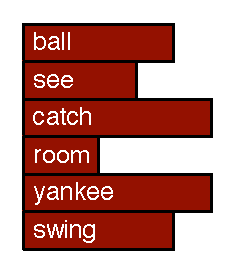
\includegraphics[width=0.7\linewidth]{spectral/shortstop}
    \column{.5\linewidth}
    The conditional probability distribution $\bar Q_{\mbox{shortshop},*}$ looks a lot like the topic distribution!
\end{columns}


\end{frame}

\begin{frame}{What about other words?}

\centering
\only<1>{
\includegraphics[width=.8\linewidth]{spectral/combination_1}}
\only<2>{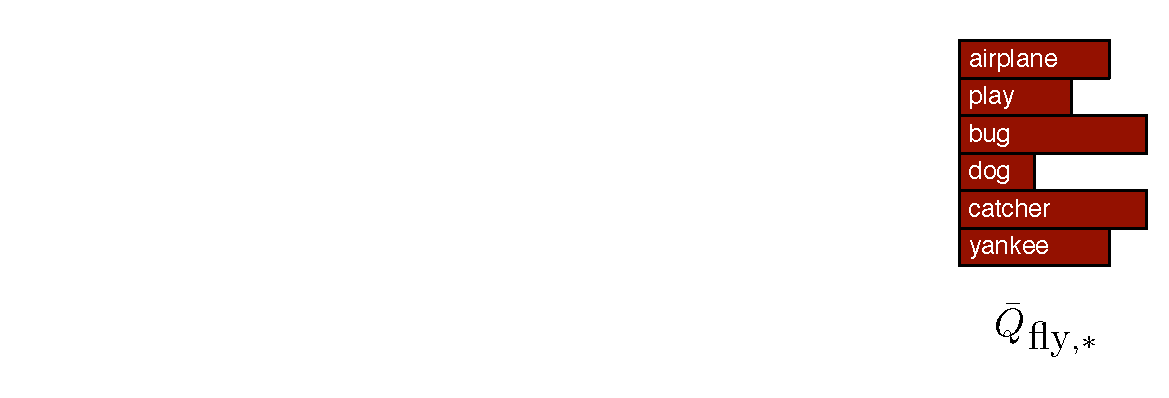
\includegraphics[width=.8\linewidth]{spectral/combination_2}}
\only<3>{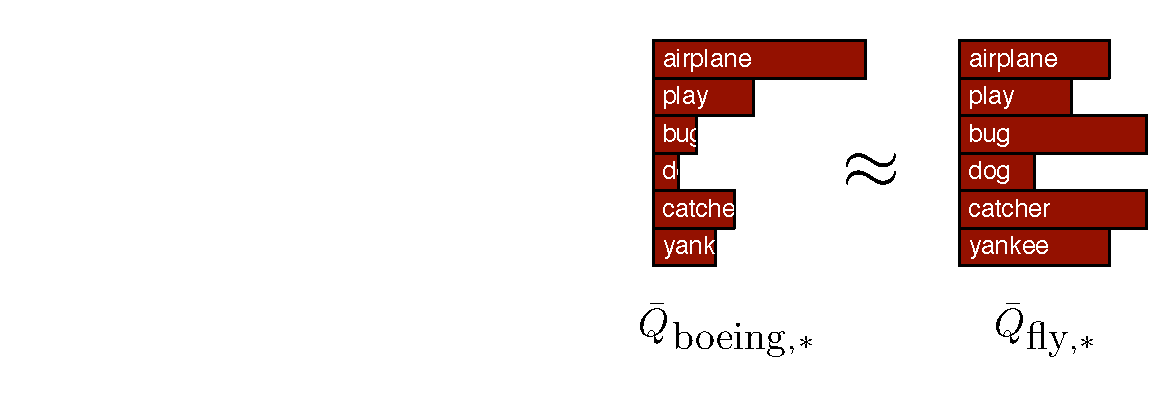
\includegraphics[width=.8\linewidth]{spectral/combination_3}}
\only<4>{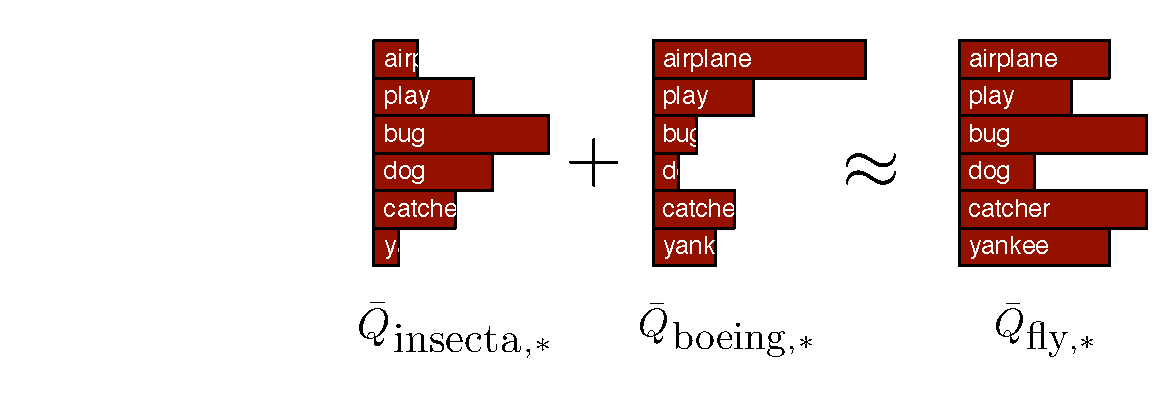
\includegraphics[width=.8\linewidth]{spectral/combination_4}}
\only<5->{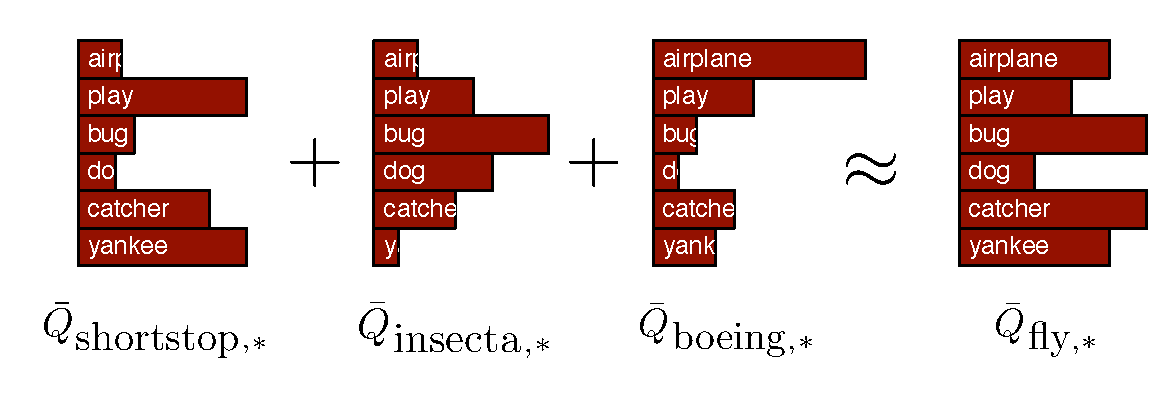
\includegraphics[width=.8\linewidth]{spectral/combination_5}}

\only<5->{
\begin{equation*}
\bar{Q}_{i,j} = \sum_{k} \alert<6>{C_{i,k}} \bar{Q}_{g_k, j}
\end{equation*}
}

\end{frame}

\begin{frame}{Topic Recovery}

\centering
\only<1>{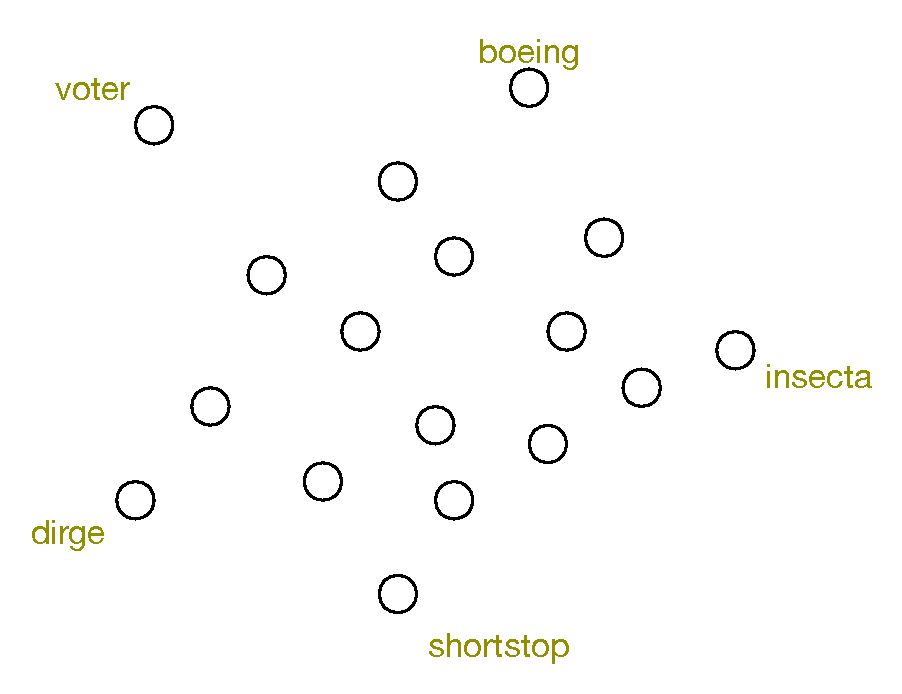
\includegraphics[width=.7\linewidth]{spectral/convex_1}}
\only<2>{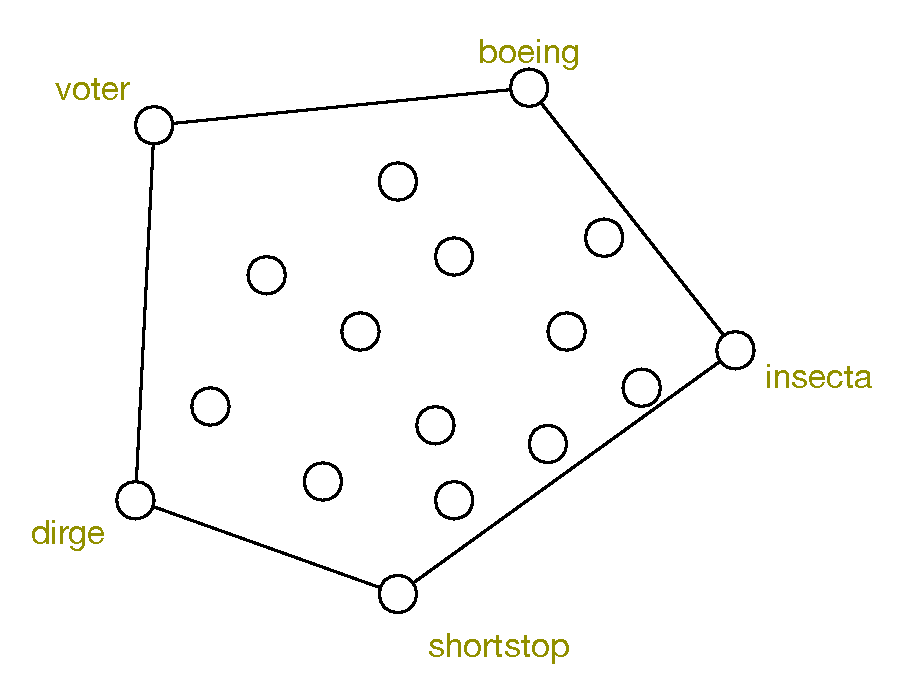
\includegraphics[width=.7\linewidth]{spectral/convex_2}}
\only<3>{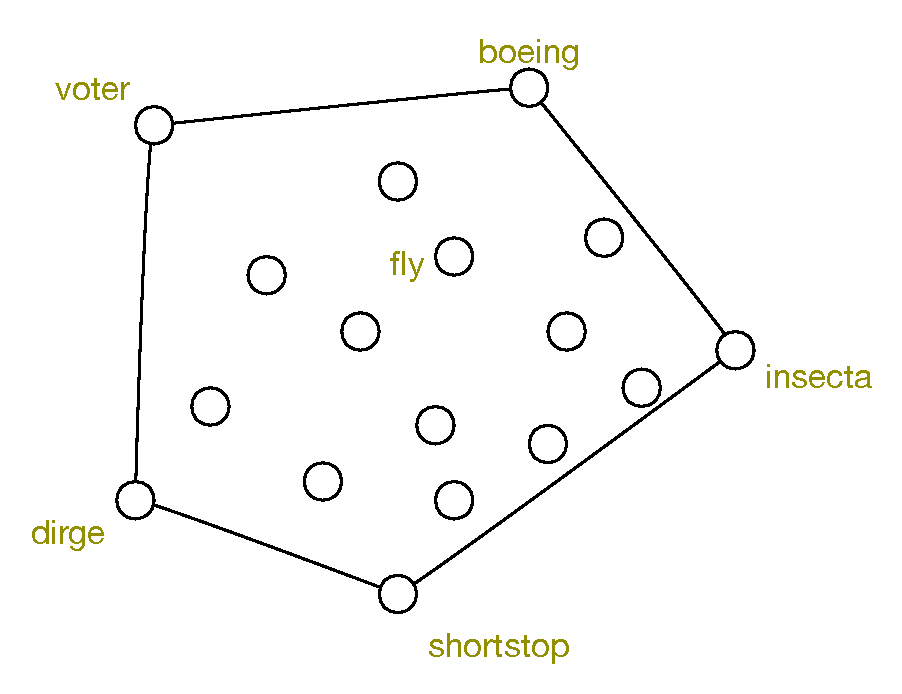
\includegraphics[width=.7\linewidth]{spectral/convex_3}}
\only<4>{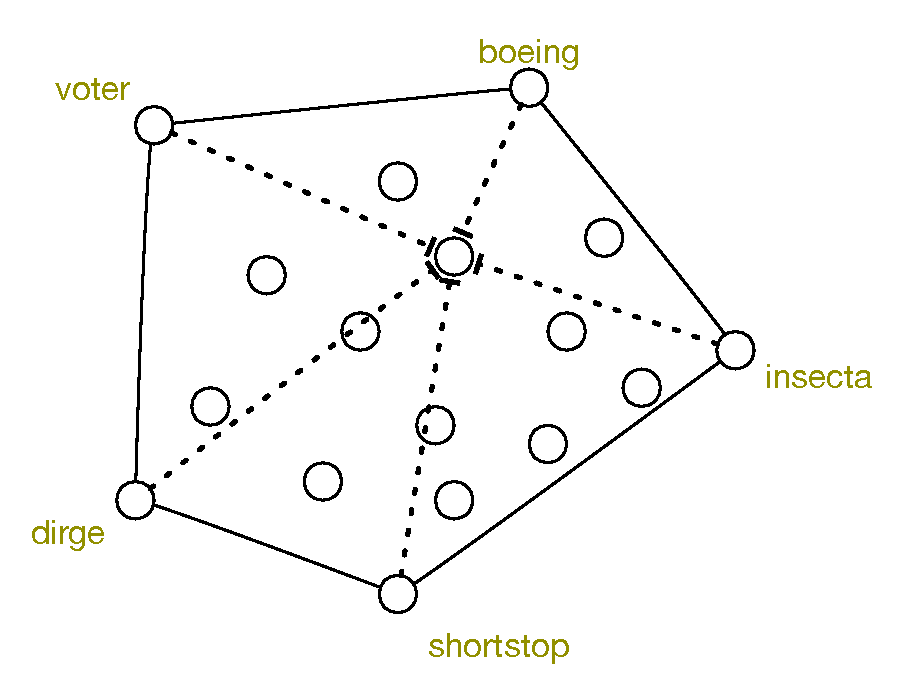
\includegraphics[width=.7\linewidth]{spectral/convex_4}}

\only<2>{ Let $g_k$ be the anchor word for topic $k$}
\only<3>{Let $C_{i,k}$ = p(topic=k $|$ word=i), $C_{i,k}\ge 0 \mbox{,
  } \sum_{k} C_{i,k} =1$ }
\only<4>{ $\bar{Q}_{i,j} = \sum_{k} C_{i,k} \bar{Q}_{g_k, j}$ }

\end{frame}

\begin{frame}{Finding Anchor Words}

  \gfx{convex_hull}{.8}

\end{frame}


\begin{frame}
\frametitle{A Significant Portion of Text is Labeled}

\begin{figure}
\centering
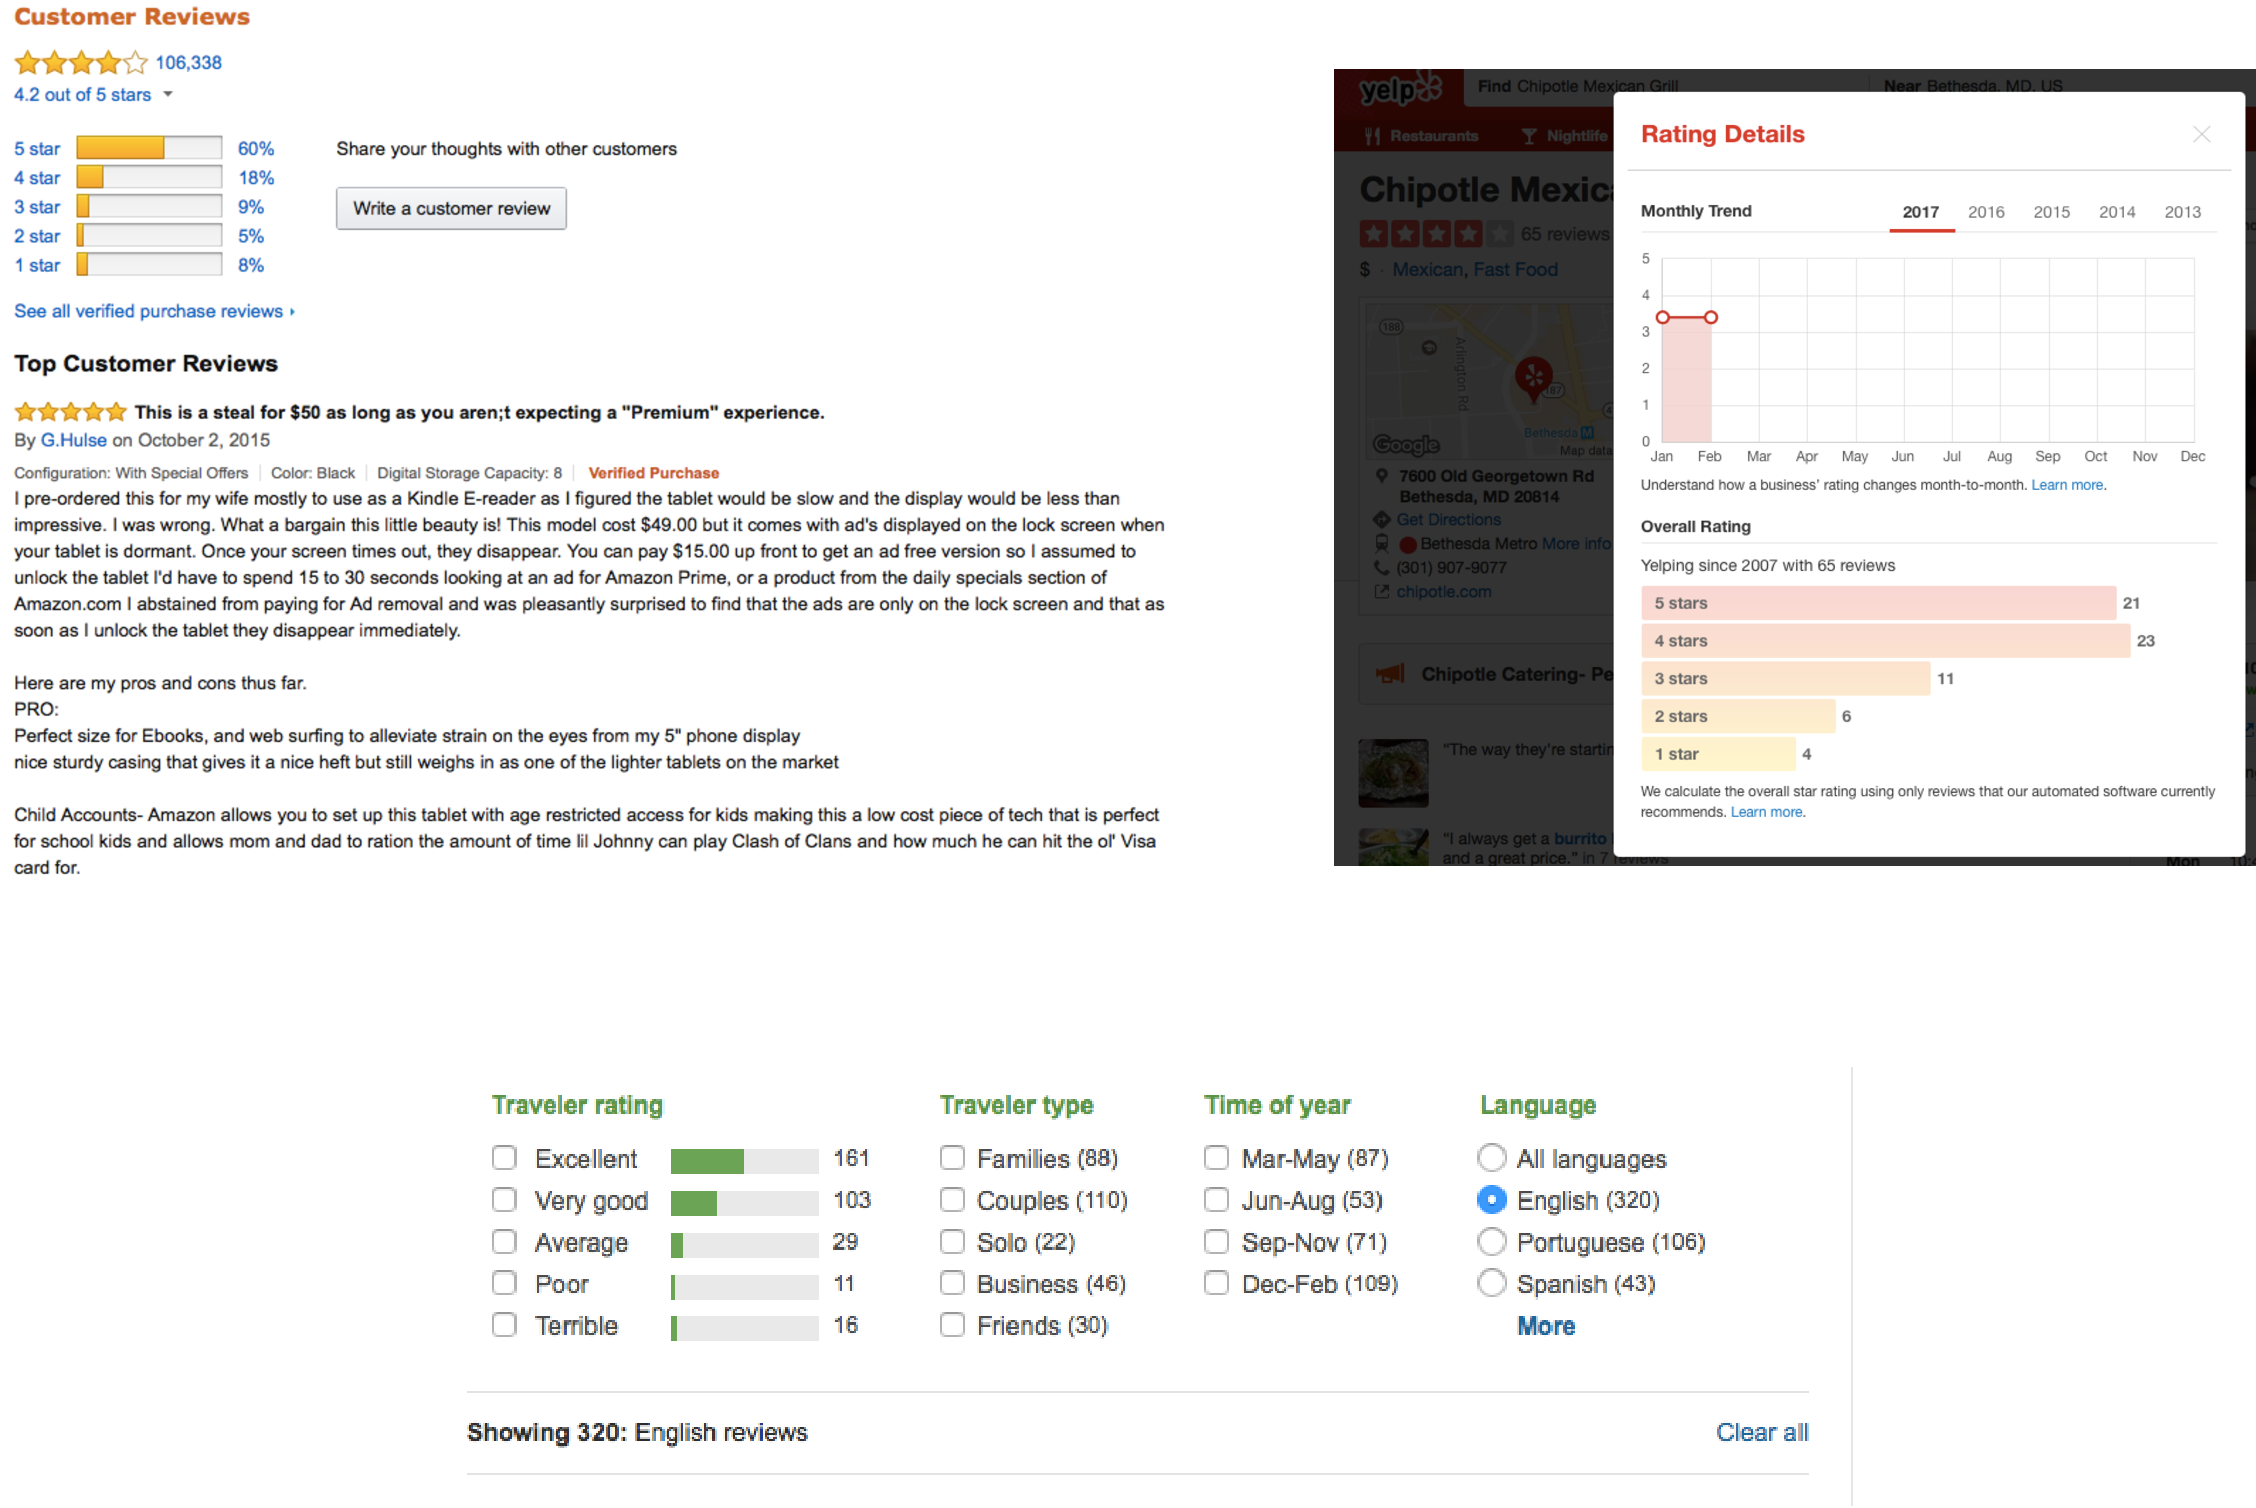
\includegraphics[width=1\linewidth]{spectral/amazon_example.pdf}
\end{figure}

\end{frame}

\begin{frame}
\frametitle{Motivation}
\begin{itemize}
\item Supervised topic models leverage latent document-level themes to capture nuanced sentiment, create sentiment-specific topics and improve sentiment prediction.
\item Examples include Supervised LDA (Blei et al., 2007),  Labelled LDA (Ramage et al., 2009), Med LDA (Zhu et al., 2009), etc.
\item The downside is sluggish performance.
\item <2-> \alert{Create a supervised model based on Anchor Words?}
\end{itemize}
\end{frame}


%\begin{frame}
%\frametitle{Contribution}
%\begin{itemize}
%\item The supervised anchor algorithm runs very fast because it inherits fast inference from the anchor algorithm.
%\item Experiments on three sentiment datasets show that supervised anchor algorithm is comparable to Supervised LDA in terms of prediction accuracy.
%\item Anchor words learned by supervised anchor algorithm provide great insight.
%%\item {\it \large{We focus on learning sentiment-specific anchor words}}. This will in turn lead to sentiment-specific topics.
%%\item Appending the conditional probability $Pr[sentiment|word]$ to word co-occurrence vector $\unsupmat{word}.$
%%\item \alert{Outcome}: we learn better topic representations and produce topics that are suitable for sentiment prediction.
%
%\end{itemize}
%\end{frame}


\begin{frame}
\frametitle{Supervised Anchor Words: \underline{Idea}}

\begin{columns}
\column{.5\linewidth}
\begin{figure}
\centering
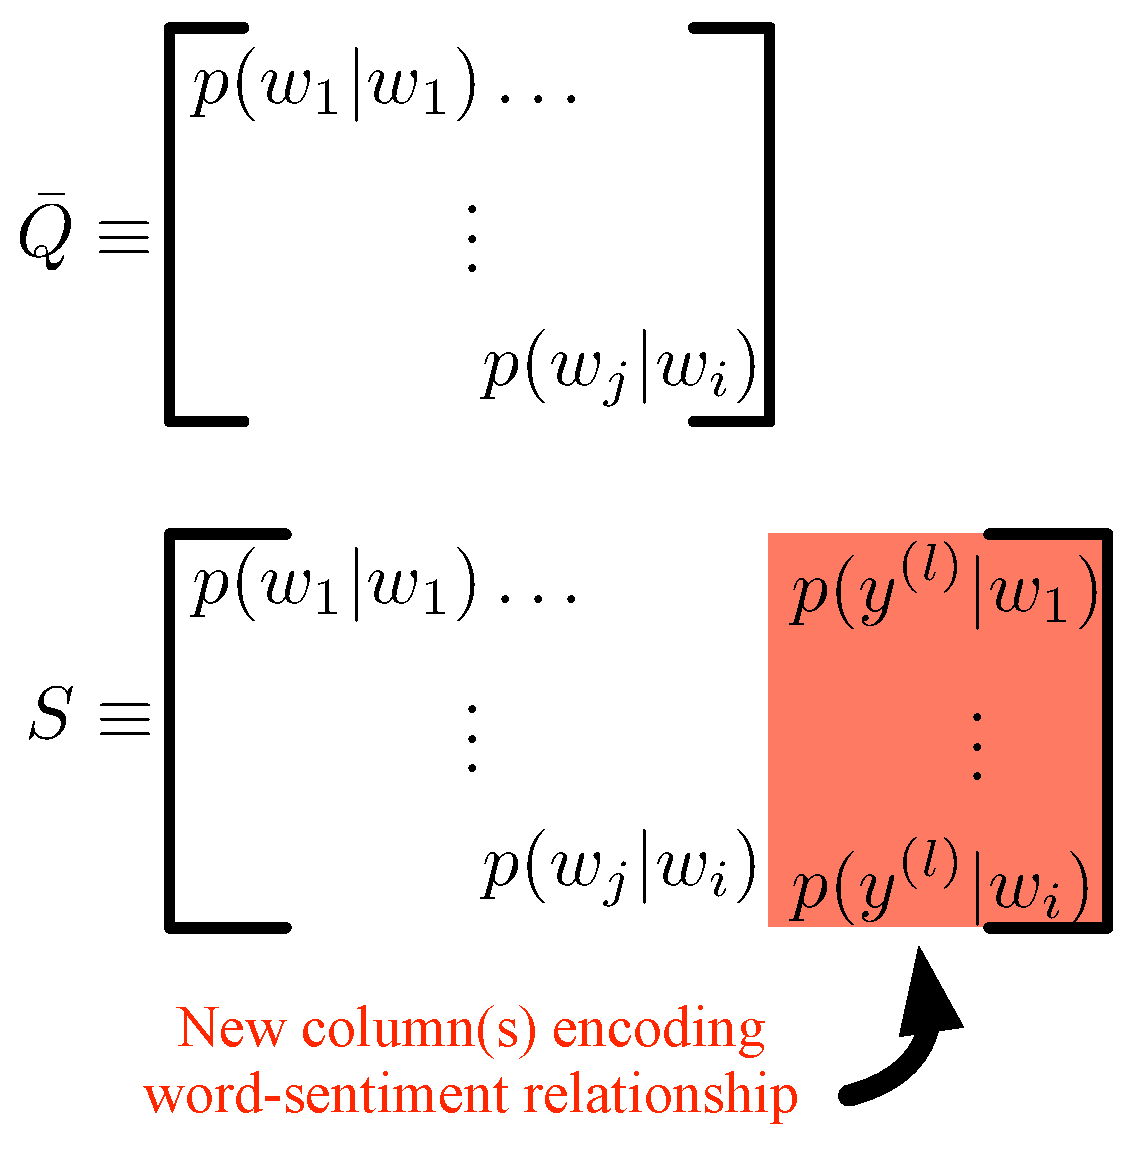
\includegraphics[width=0.9\linewidth]{spectral/augmented_matrix.pdf}
\end{figure}

\column{.5\linewidth}
\begin{equation*}
  \suprow{i} = \sum_{g_k \in \mathcal{G}} \coef{i,k} \suprow{g_k} .
\label{eq:lincomb-2}
\end{equation*}
\end{columns}
\end{frame}

%\begin{frame}
%\frametitle{Supervised Anchor Words}
%
%%\begin{equation}
%%S_{i,(V+l)} \equiv \frac{\sum_{d} ( \ind{i \in d} \cdot \ind{y_d = y^{(l)}} ) }{
%%  \sum_{d} \ind{i \in d}} .
%%\label{eq:labelest}
%%\end{equation}
%
%\begin{itemize}
%\item {\it \large{We focus on learning sentiment-specific anchor words}}. This will in turn lead to sentiment-specific topics.
%%\item  We explicitly represent the combination of words and discrete sentiment values by a
%\item <2->Appending the conditional probability $Pr[sentiment|word]$ to word co-occurrence vector $\unsupmat{word}.$
%\item <3->\alert{Outcome}: we learn better topic representations and produce topics that are suitable for sentiment prediction.
%\end{itemize}
%
%\end{frame}


\begin{frame}
\frametitle{Supervised Anchor Words: \underline{Intuition}}

%\begin{figure}
\centering
\begin{columns}
\column{.5\linewidth}
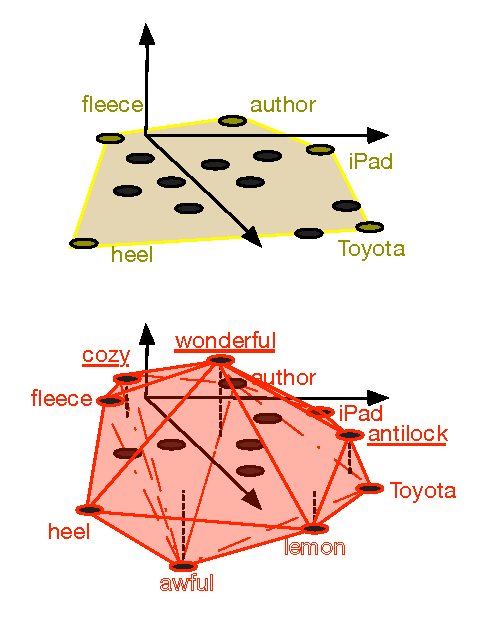
\includegraphics[width=0.9\linewidth]{spectral/jutting_anchors.pdf}
%\captionsetup{margin={.5cm,0cm}}%justification=centering}
%  \caption{\normalsize{Adding an additional dimension to capture sentiment changes
%    the convex hull: positive words appear above the original 2D
%    plane (underlined) and negative words appear below (in outline).}}
%  \label{fig:jutting-anchors}
%\end{figure}
\column{.5\linewidth}
\begin{itemize}
%\item Anchor words form a convex hull that encloses all other words in the vocabulary.
\item Adding sentiment related dimensions moves words UP or DOWN
\item forming sentiment-specific points
\item possibility of having different anchor words
\end{itemize}
\end{columns}
\end{frame}

\begin{frame}
\frametitle{Evaluation of Supervised Anchor Words}

\begin{itemize}
\item {\bf \large{Goal}}: Evaluate the new topics generated by the proposed model in a prediction task. We focus on binary classification in sentiment analysis datasets.
\item Sentiment datasets.
\begin{table}
   \begin{center}
    \normalsize
   \begin{tabular}{c c c c c c}
   \hline\hline
\rule{0pt}{2ex}
   Corpus&Train&Test&Tokens& Vocab& {\bf \textsc{+1}}  \\
   \hline
\rule{0pt}{2ex}
   \abr{amazon} & 13,300 & 3,314 &1,031,659&2,662  & 52.2\% \\
    \abr{tripadvisor}   & 115,384 & 28,828 &12,752,444&4,867 & 41.5\% \\
  \abr{yelp} &  13,955 & 3,482 & 1,142,555 &2,585&27.7\% \\
   \hline
   \end{tabular}
 \end{center}
%\vspace{0.2cm}
% \caption{\normalsize{Statistics for the datasets employed in the experiments.}}
%   \label{tab:corpus}
\end{table}
\end{itemize}

\end{frame}

\begin{frame}
\frametitle{Runtime Analysis}

\begin{figure}
\centering
%\captionsetup{margin={.5cm,0cm}}%justification=centering}
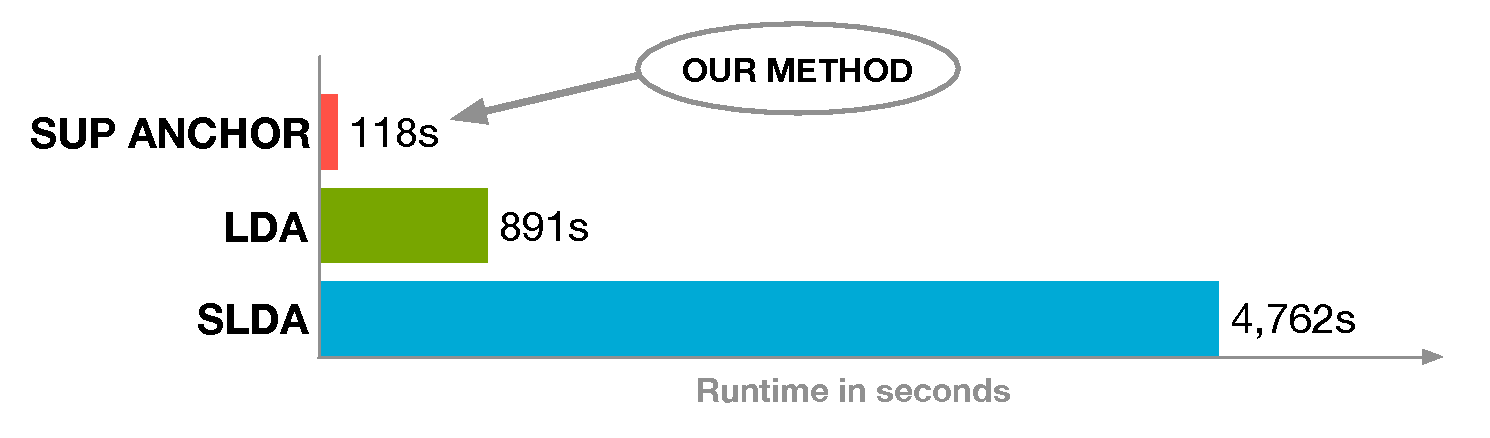
\includegraphics[width=\linewidth]{spectral/amazon_time.pdf}
%\caption{\normalsize{Total time for training and prediction on \abr{amazon} dataset; \sank{} takes much less time than \slda{}.}}
\end{figure}
\begin{itemize}
\item Total time for training and prediction on \abr{amazon} dataset.
%; \sank{} takes much less time than \slda{}.
\end{itemize}
\end{frame}


%\begin{frame}
%\frametitle{Prediction Accuracy \& Topic Interpretability}
%\begin{itemize}
%\item For prediction accuracy, \sank{} consistently outperforms all other models on all sentiment datasets.
%\item \sank{} has comparable topic interpretability (Lau et al., 2014, NPMI) to \ank{}.
%\item Nguyen et al., 2014 show that with regularization anchor algorithms can produce comparable topics with those produced by \lda{}.
%\end{itemize}
%
%\end{frame}

\begin{frame}
\frametitle{Prediction Accuracy}
\begin{figure}
\centering
%\captionsetup{margin={.5cm,0cm}}%justification=centering}
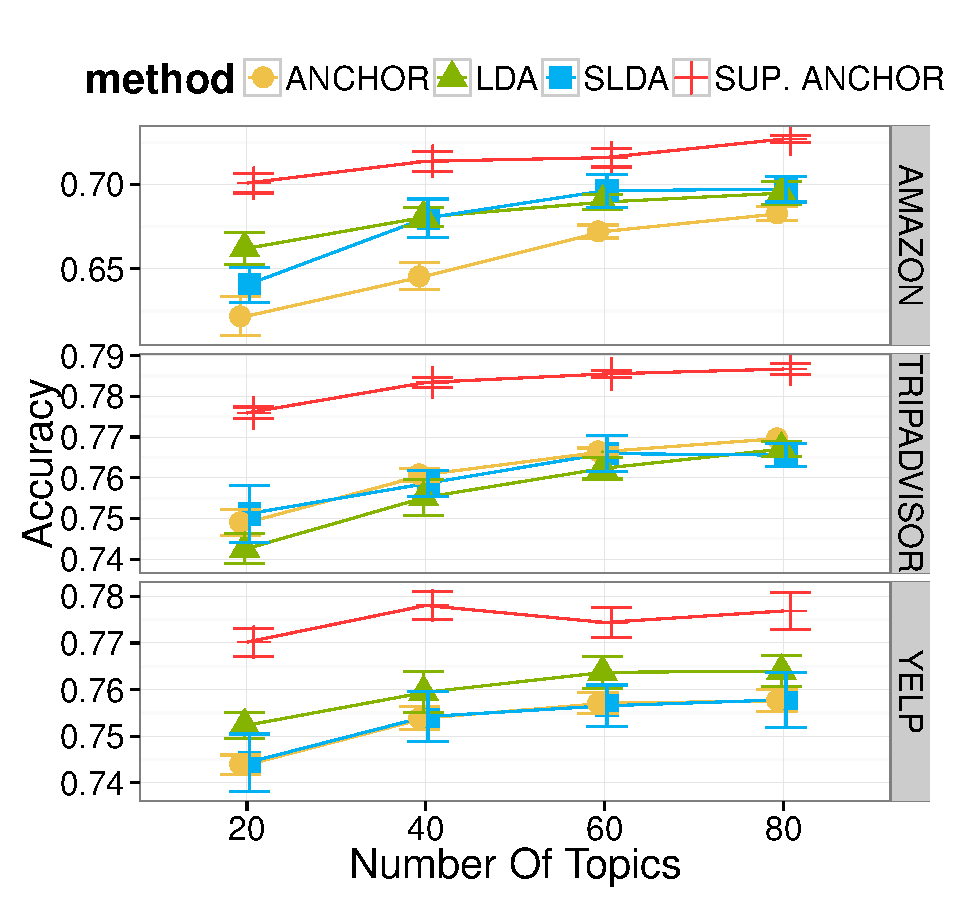
\includegraphics[width=0.65\linewidth]{spectral/test_accuracy_ERROR.pdf}
%\caption{\normalsize{\sank{} outperforms \ank{}, \lda{}, and \slda{} on all three datasets.}}%The results are based on \abr{logistic} as it produces the best accuracy consistently for \ank{}, \sank{}, and \lda{}.}}
%\label{fig:test-accuracy}
\end{figure}

\end{frame}

\begin{frame}
\frametitle{Topic Coherence}
\begin{figure}
\centering
%\captionsetup{margin={.5cm,0cm}}%justification=centering}
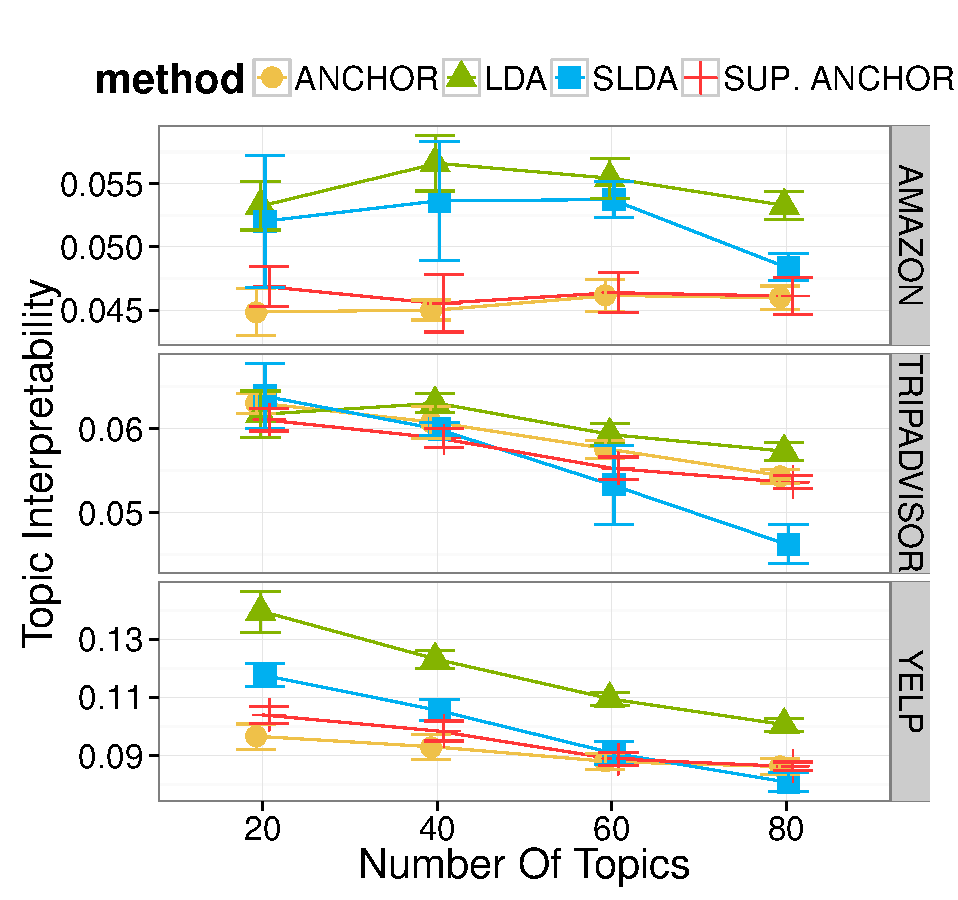
\includegraphics[width=0.65\linewidth]{spectral/topic_coherence_ERROR.pdf}
%\caption{\normalsize{\sank{} and \ank{} produce the same topic quality. \lda{} produces the best topics.}}
\end{figure}

\end{frame}


\begin{frame}
\frametitle{Anchor Words and Their Topics}
%\begin{itemize}
%\item  \sank{} produces anchor words around the same strong
%lexical cues that could discover better sentiment topics (e.g. positive reviews mentioning a {\it \large{favorite}} restaurant or negative reviews complaining about {\it \large{long waits}}).
%\end{itemize}
\begin{figure}
\centering
%\captionsetup{margin={.5cm,0cm}}%justification=centering}
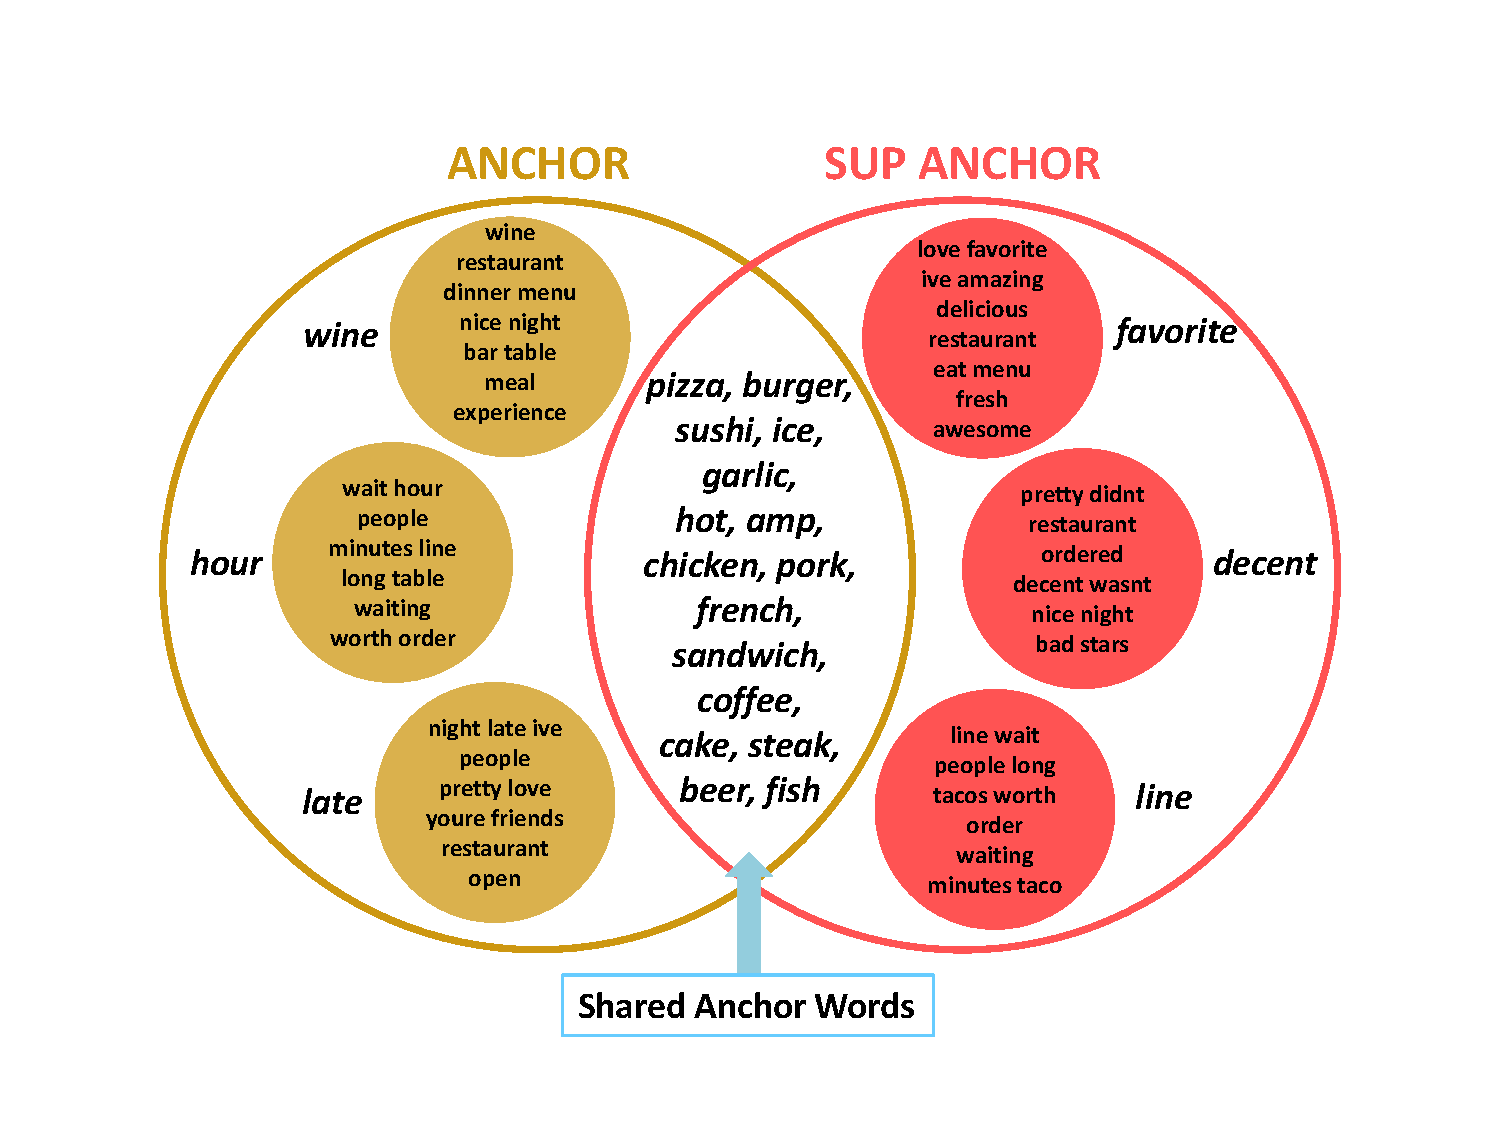
\includegraphics[width=0.8\linewidth]{spectral/venn_colors.pdf}
%\vspace{0.3cm}
%\caption{\normalsize{Topics generated for the \abr{yelp} dataset: anchor
%  words shared by both \ank{} and \sank{} are listed. The distinct anchor words reflect positive (``favorite'') and negative (``line'') sentiment rather than less sentiment-specific qualities of restaurants (e.g., restaurants open ``late'').}}
\end{figure}

\end{frame}

\begin{frame}{Ongoing Work}

  \begin{itemize}
    \item Near-instant updates
    \item Using multiple anchor words can improve coherence (and add interactivities)
    \item Downside: hard to create new models
    \item Hard to debug
  \end{itemize}

\end{frame}


\end{document}
